\documentclass[12pt,a4paper]{article}
\usepackage[utf8]{inputenc}
\usepackage[T1]{fontenc}
\usepackage{amsmath,amssymb,bm}
\usepackage{geometry}
\usepackage{graphicx}
\usepackage{xcolor}
\usepackage{tikz}
\usepackage{enumitem}
\usepackage{hyperref}
\usepackage{tcolorbox}
\usepackage{fancyhdr}
\usepackage{booktabs}
\usepackage{float}
\usepackage{caption}
\usepackage{subcaption}
\usepackage{pgfplots}

\geometry{margin=2.5cm}
\setlength{\headheight}{14.5pt}
\hypersetup{colorlinks=true,linkcolor=blue,citecolor=blue,urlcolor=blue}
\pgfplotsset{compat=1.18}

\newtcolorbox{resultbox}[1][]{colback=green!5!white,colframe=green!50!black,fonttitle=\bfseries,title=#1}

\pagestyle{fancy}
\fancyhf{}
\fancyhead[L]{\textbf{HW7 --- Computed Torque Control}}
\fancyhead[R]{June 2026}
\fancyfoot[C]{\thepage}

\title{\textbf{Homework 7: Computed Torque Control of a 4-DOF Manipulator}}
\author{}
\date{}

\begin{document}
\maketitle
\vspace{-15pt}

\begin{center}
\small
\textbf{Manipulator:} 3R+1P (MLS Example 4.4).~~Link lengths: $l_1=0.9$\,m, $l_2=0.7$\,m, $l_0=0.3$\,m.~~
Masses: 35, 25, 18, 7\,kg.~~
$\bm{\beta}=[0.9,0.45,0.4,0.9]$.~~
$\bm{\theta}(0)=[0.3\pi,0.2\pi,0.35\pi,-0.03]^\top$.\\
\textbf{Desired final values:} $[2,1,0.5,0.08]^\top$ (rad / m).~~
\textbf{Gains:} $\mathbf{K}_p=2500\mathbf{I}$, $\mathbf{K}_v=100\mathbf{I}$ ($\omega_n=50$\,rad/s, $\zeta=1$).~~
\textbf{Saturation:} $|\bm{\tau}|\le[6000,2000,1000,100]^\top$.
\end{center}

% ===================================================================
\section{Part (a): Computed Torque Controller}
% ===================================================================

\textbf{Method.} The computed torque law $\bm{\tau}=\mathbf{M}(\bm{\theta})\ddot{\bm{\theta}}^*+\mathbf{C}\dot{\bm{\theta}}+\mathbf{N}$ with $\ddot{\bm{\theta}}^*=\ddot{\bm{\theta}}_d+\mathbf{K}_v\dot{\mathbf{e}}+\mathbf{K}_p\mathbf{e}$ exactly cancels the nonlinear dynamics, yielding linear error dynamics $\ddot{\mathbf{e}}+\mathbf{K}_v\dot{\mathbf{e}}+\mathbf{K}_p\mathbf{e}=\mathbf{0}$. The desired trajectory is a quintic rounded step starting at $t_0=1.0$\,s with $\Delta t=0.4$\,s, scaling a unit step to the specified amplitudes. Dynamics are computed via screw theory (PoE) in \texttt{MCNsim}.

\textbf{Results.}

\begin{figure}[H]
\centering
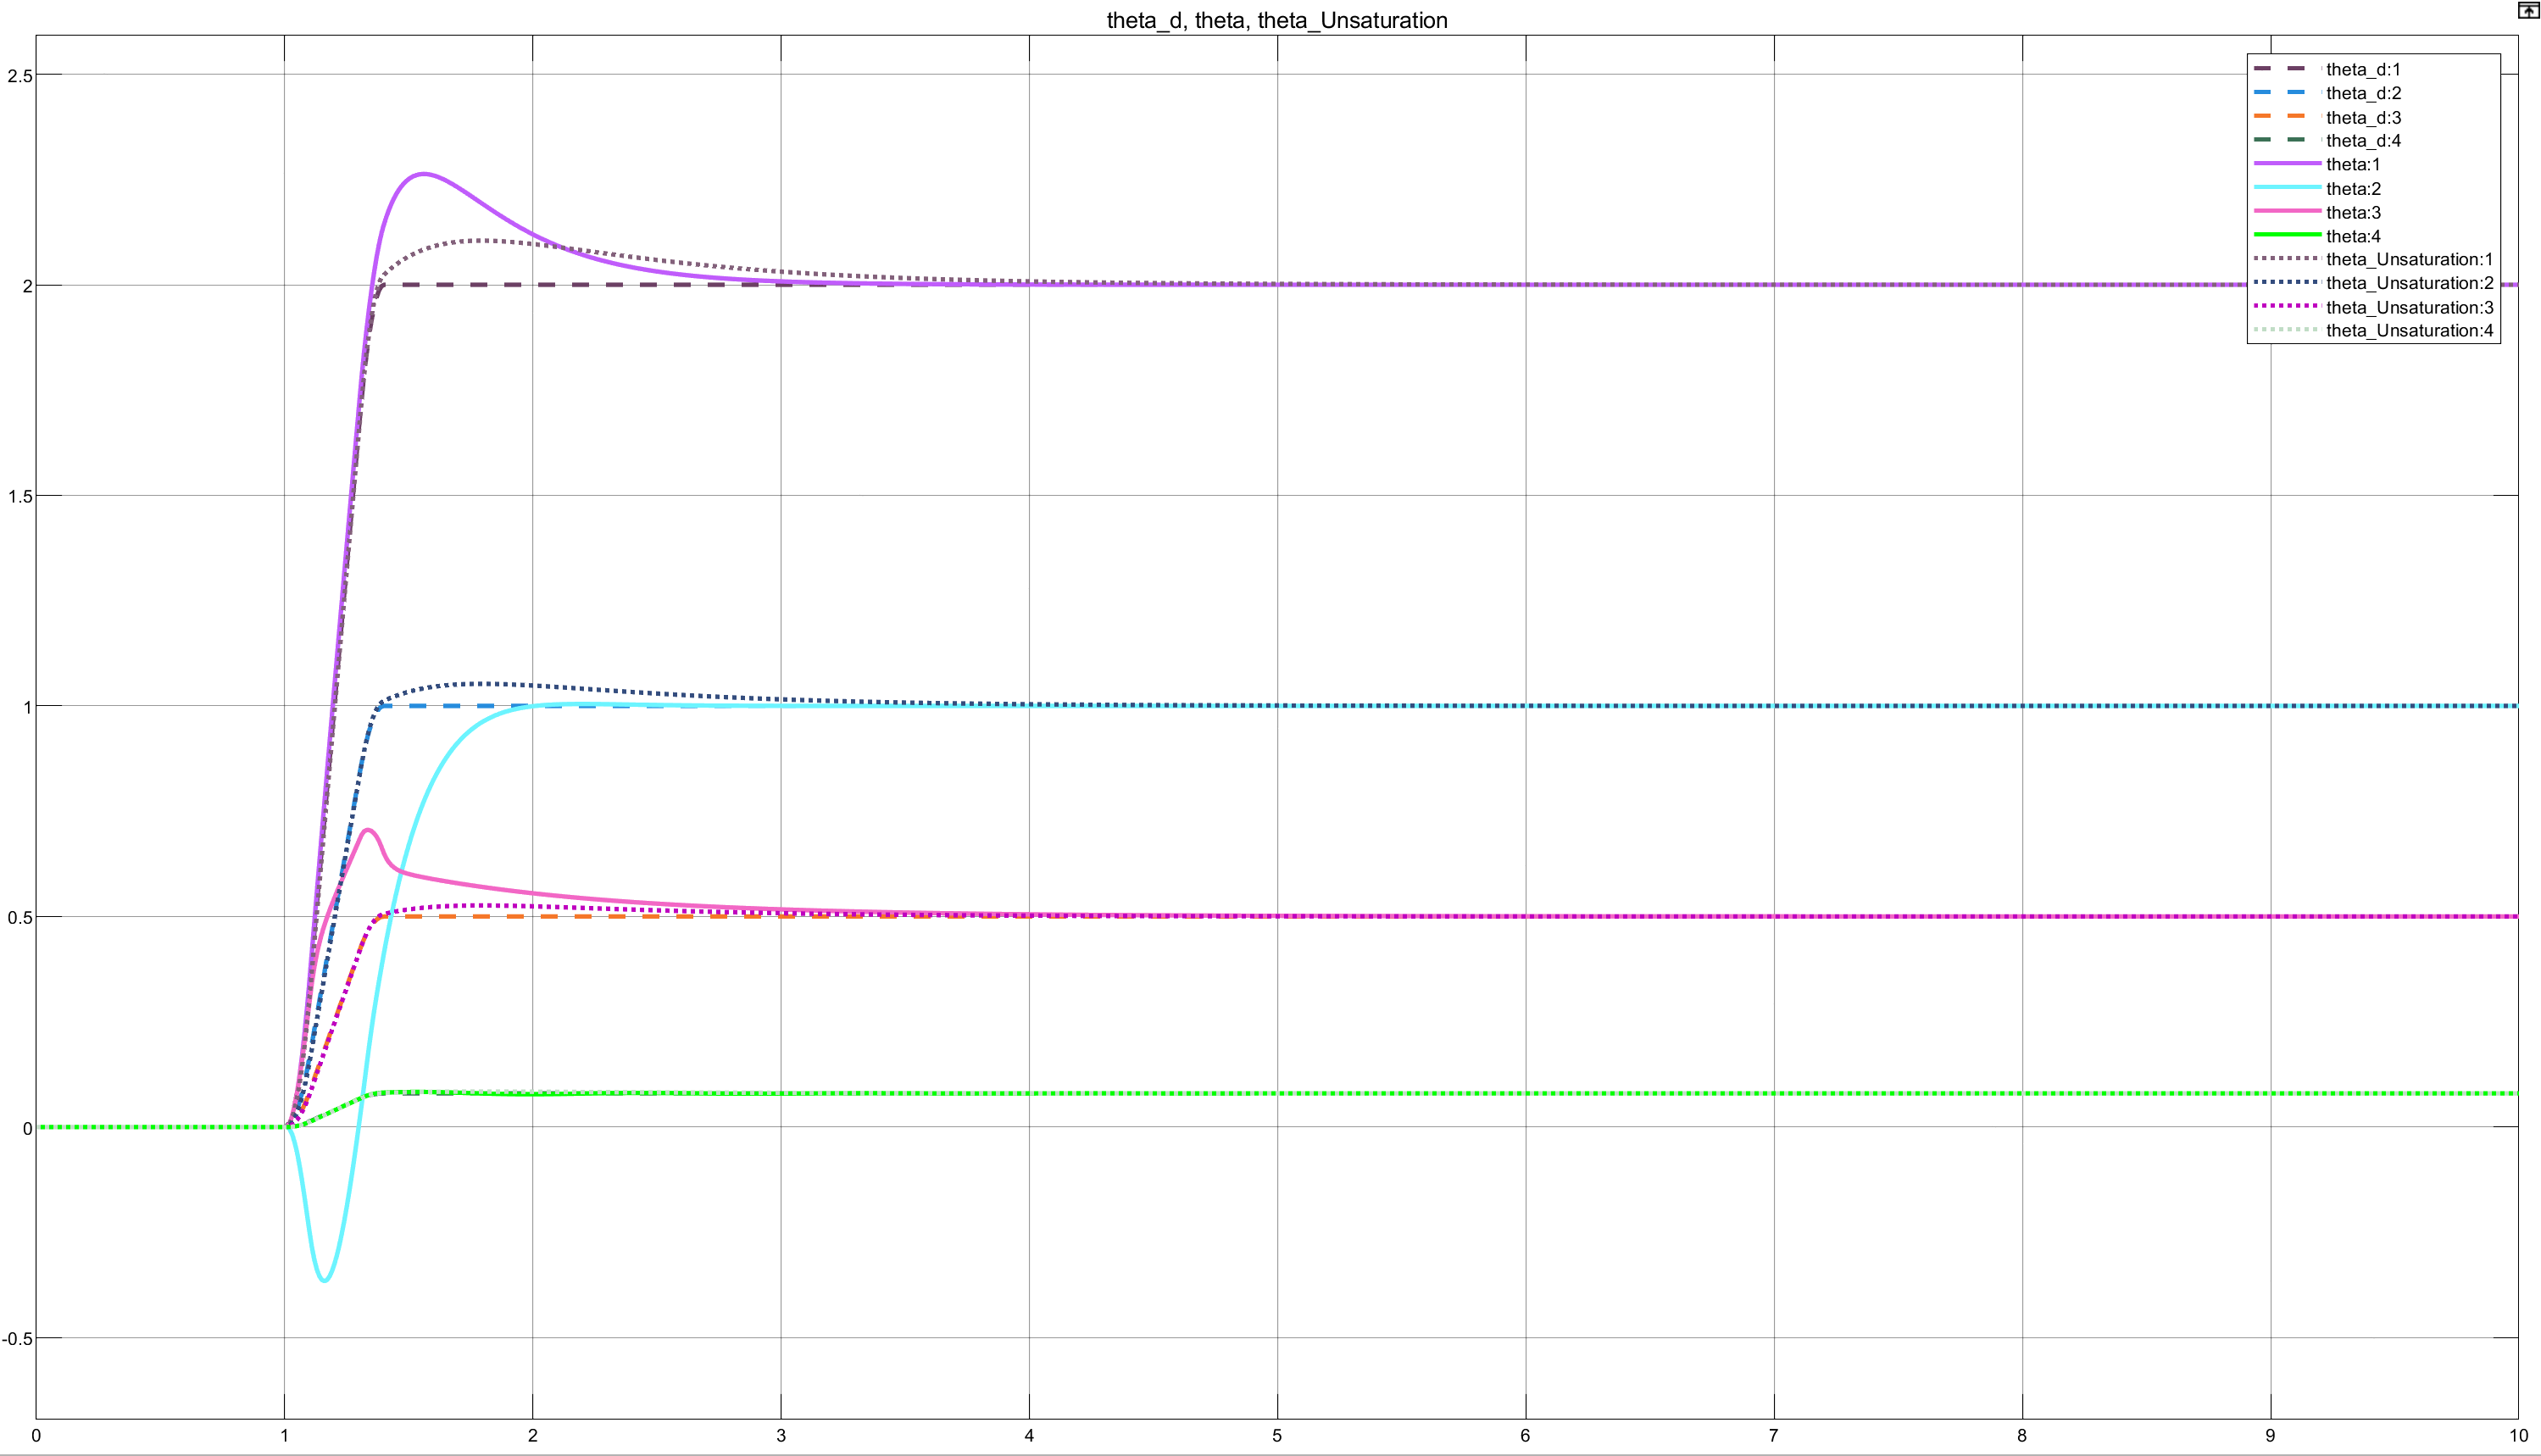
\includegraphics[width=0.92\textwidth]{a_theta.png}
\caption{Nominal computed torque tracking. \textbf{Dashed:} $\bm{\theta}_d$ (desired). \textbf{Solid:} $\bm{\theta}$ (actual, with saturation). \textbf{Dash-dot:} $\bm{\theta}_{\text{unsat}}$ (without saturation).}
\label{fig:a_theta}
\end{figure}

\begin{figure}[H]
\centering
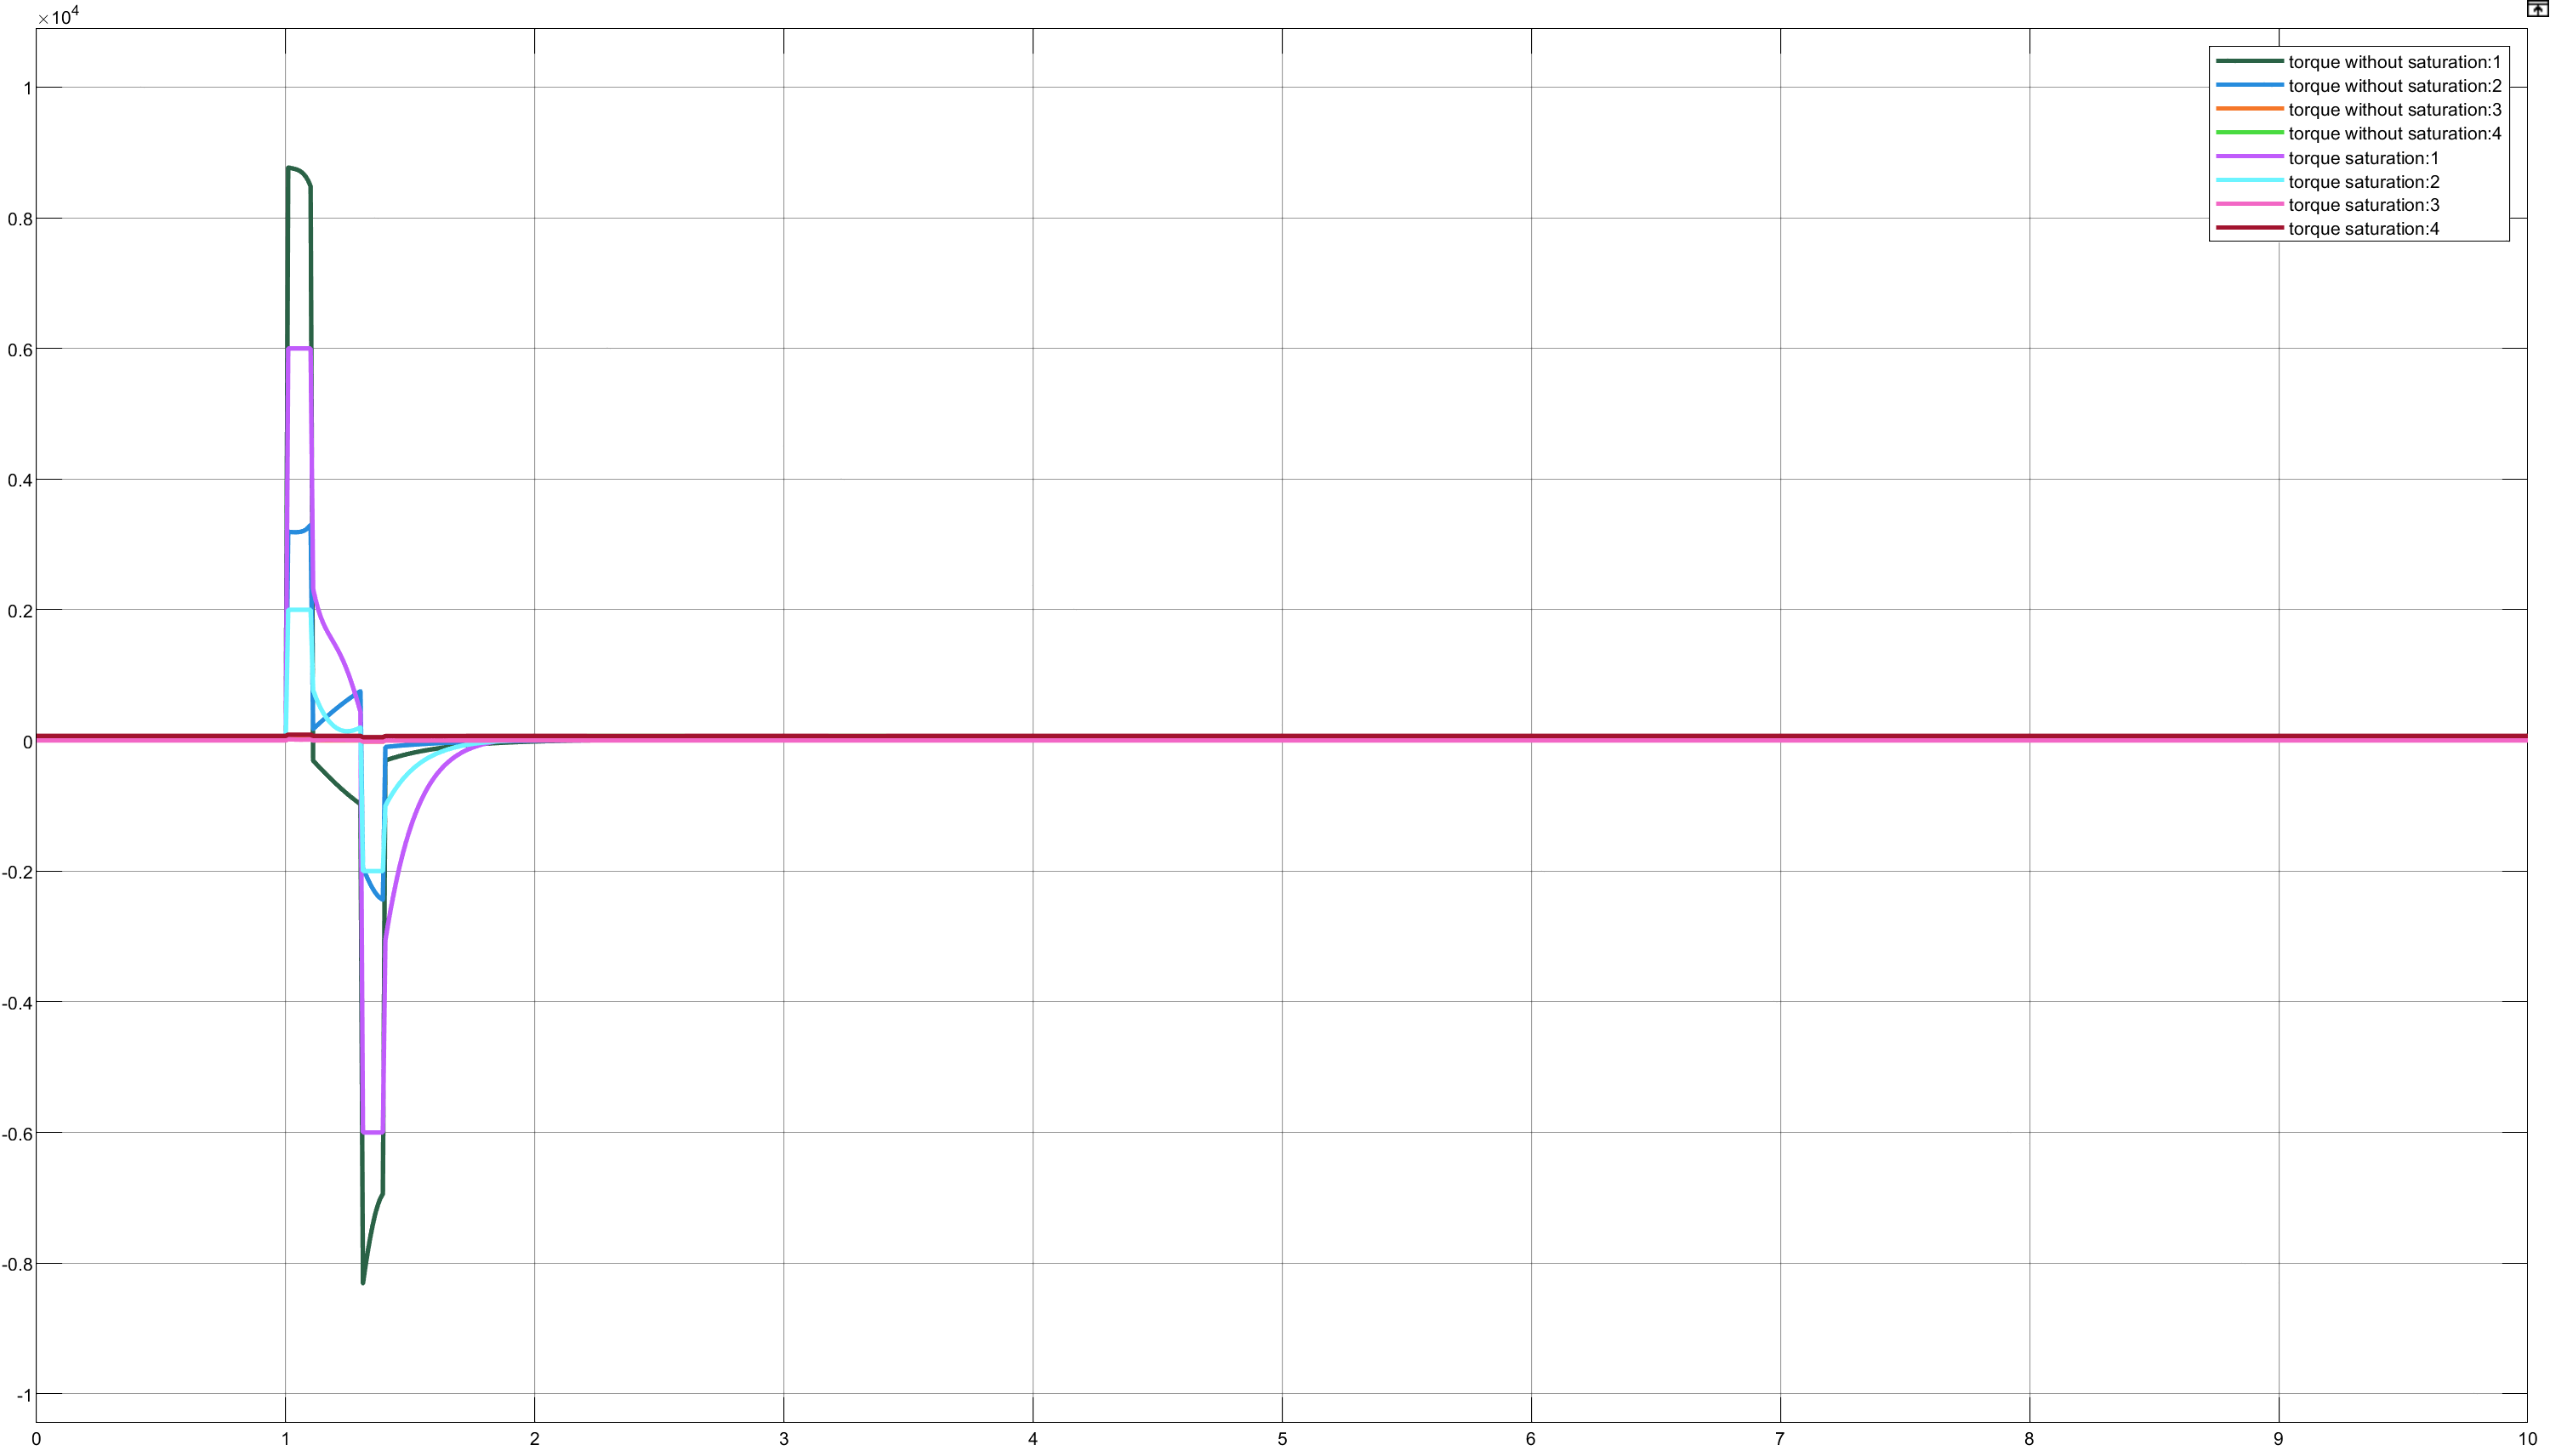
\includegraphics[width=0.93\textwidth]{a_torque.png}
\caption{Control torques $\bm{\tau}(t)$ with saturation limits $[6000,2000,1000,100]^\top$ shown.}
\label{fig:a_torque}
\end{figure}

\begin{resultbox}
\textbf{Observations:}
\begin{itemize}[nosep]
  \item All joints converge to desired values: $\theta_1\to2$, $\theta_2\to1$, $\theta_3\to0.5$\,rad, $d_4\to0.08$\,m.
  \item Errors converge exponentially ($\tau\approx0.02$\,s) to zero --- exact cancellation yields perfect asymptotic tracking.
  \item Saturation has a visible effect: $\bm{\theta}$ (with saturation) deviates from $\bm{\theta}_{\text{unsat}}$ (without saturation), most notably on joint~2 where a temporary dip occurs --- indicating that the torque limits $[6000,2000,1000,100]^\top$ are occasionally hit during the transient (see also \S\ref{sec:d}).
  \item Torque peaks during step transition $t\in[1,1.4]$\,s; joint~1 requires the largest torque.
\end{itemize}
\end{resultbox}

% ===================================================================
\section{Part (b): Robustness to Parameter Mismatch}
% ===================================================================

\textbf{Method.} We perturb the plant spatial inertias by $\delta\in\{-10\%,-5\%,+5\%,+10\%\}$ while keeping the controller at nominal values --- simulating aging-induced parameter drift. Saturation limits $[6000,2000,1000,100]^\top$ are active. Figure~\ref{fig:b} shows the case $\delta=+10\%$ (plant heavier by 10\%).

\textbf{Results.}

\begin{figure}[H]
\centering
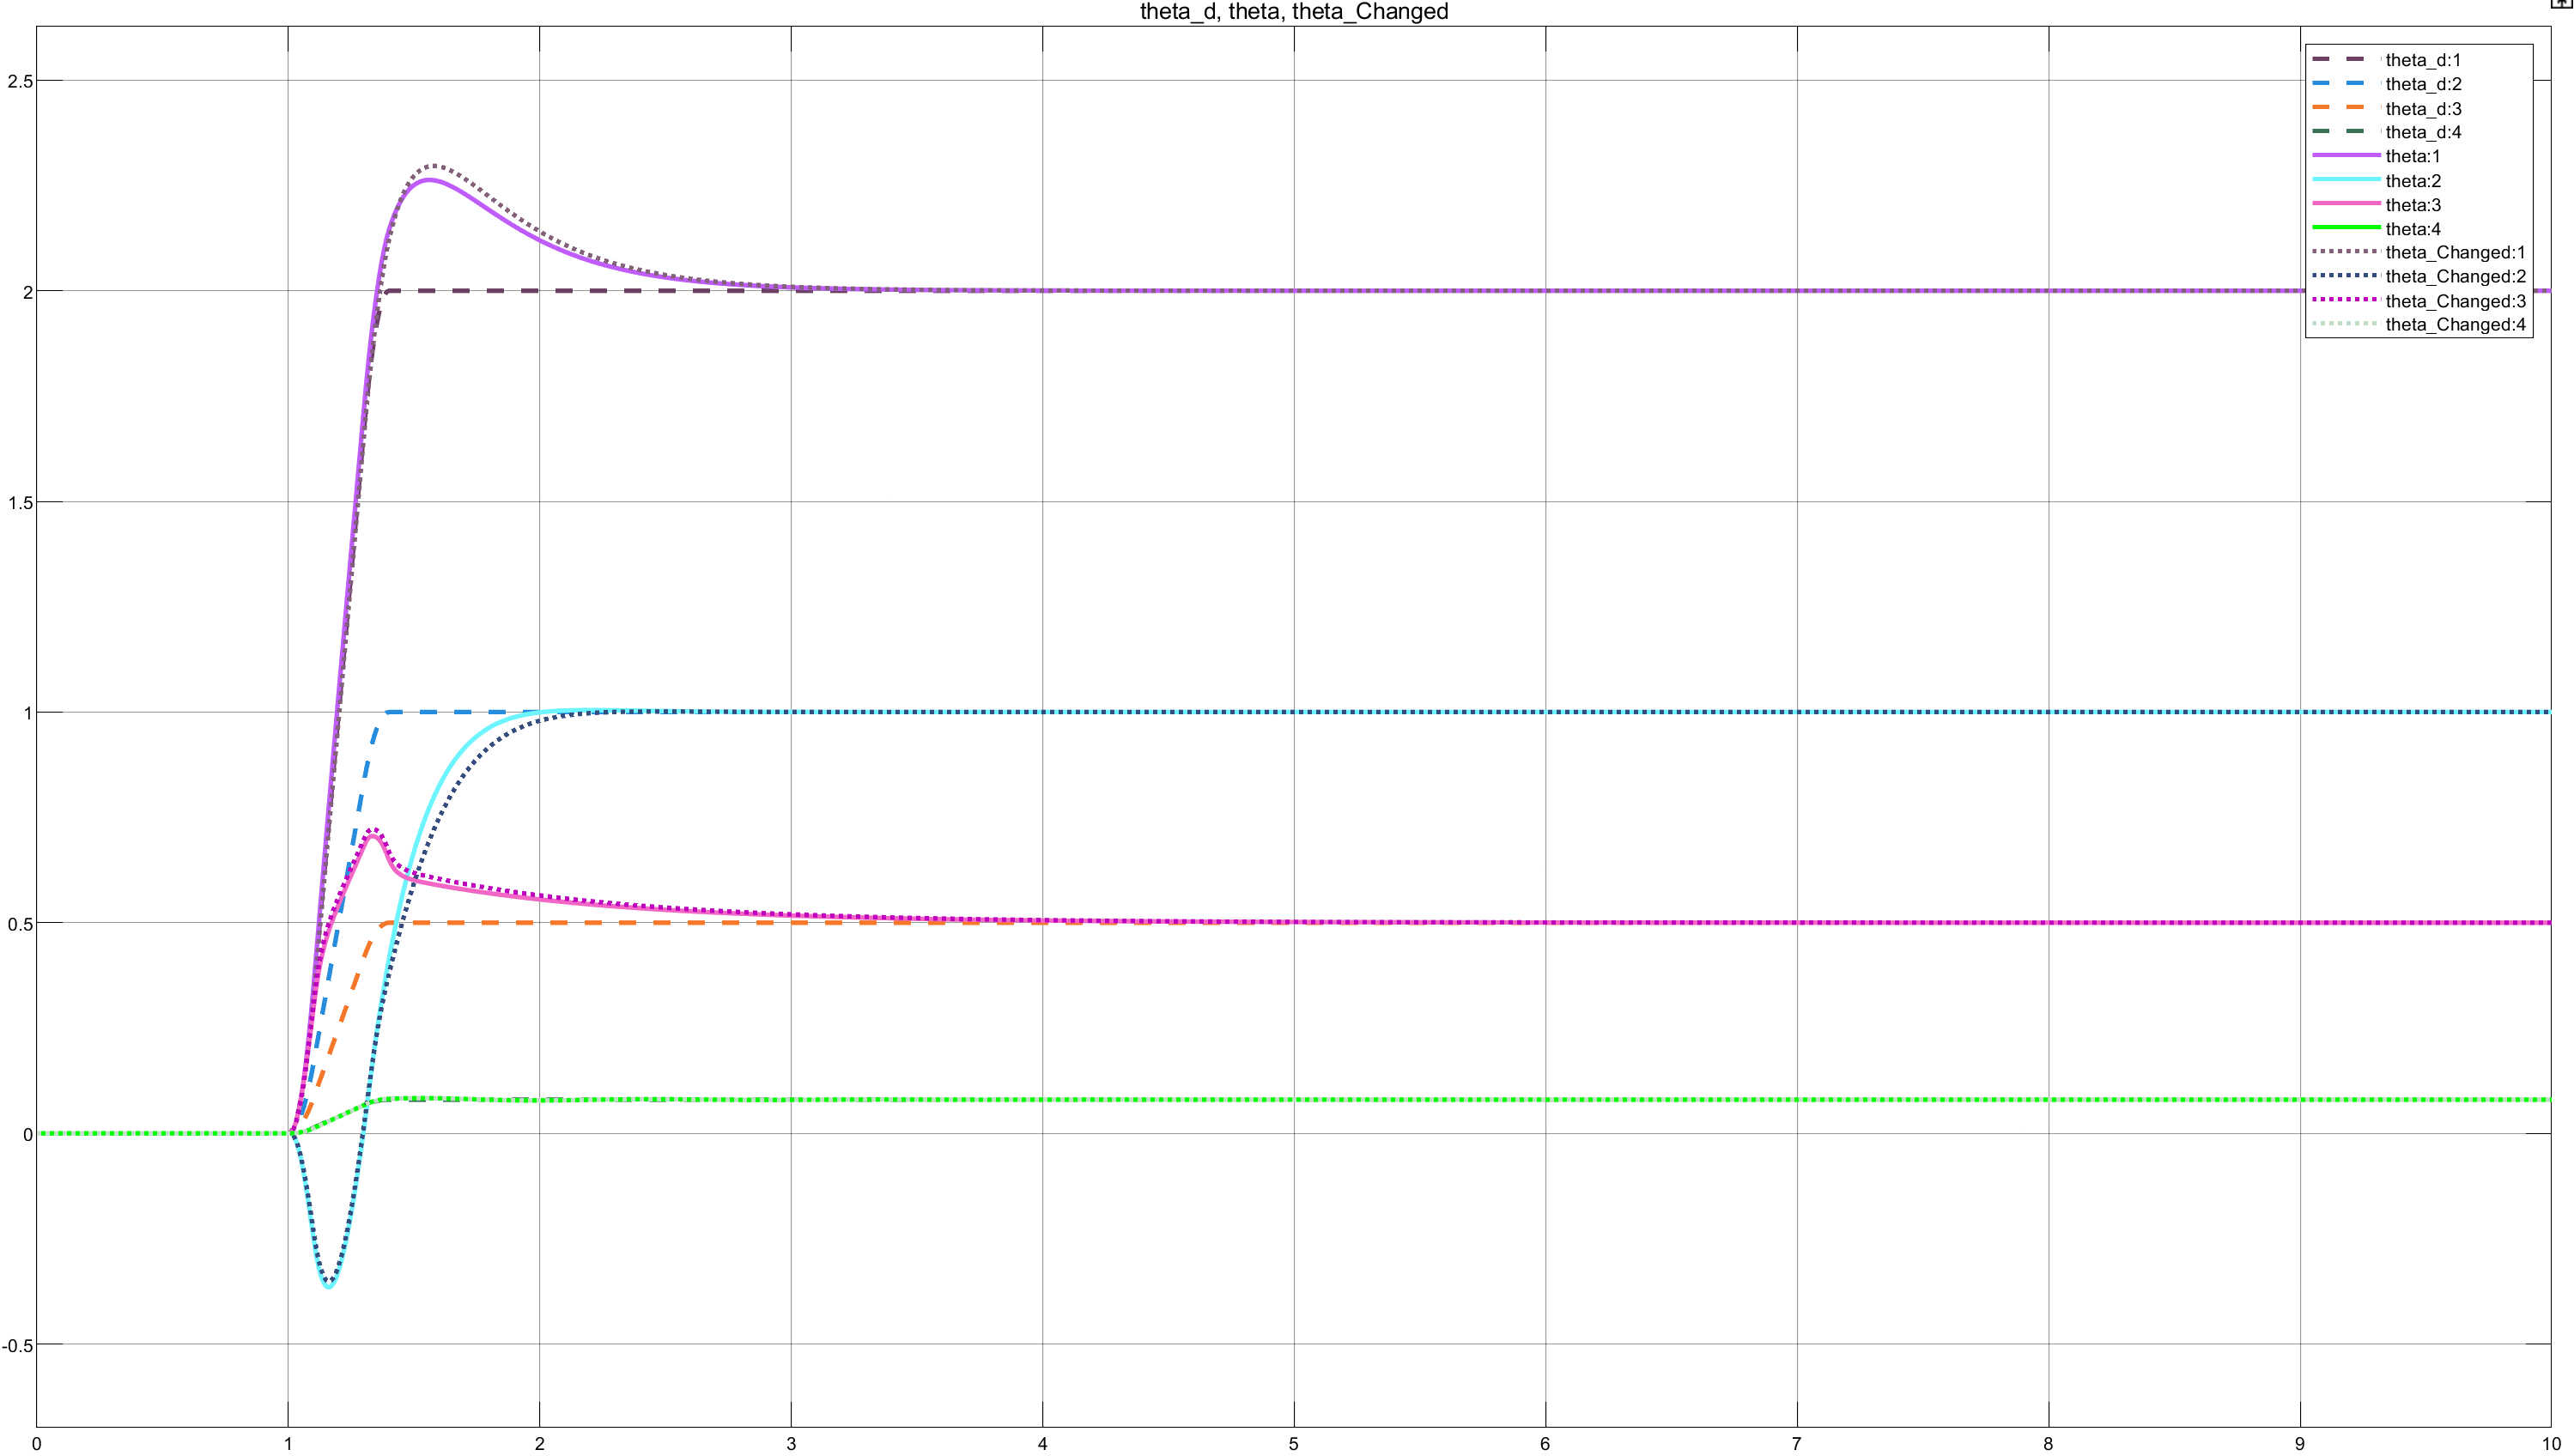
\includegraphics[width=0.92\textwidth]{b.png}
\caption{Robustness under parameter perturbation: $\delta=+10\%$ (plant $\hat{\mathbf{M}}_i^s$ multiplied by $1.1$), controller unchanged. Saturation limits active.}
\label{fig:b}
\end{figure}

\begin{resultbox}
\textbf{Observations (Fig.~\ref{fig:b}, $\delta=+10\%$ with saturation):}
\begin{itemize}[nosep]
  \item Despite the plant being 10\% heavier (simulating aging), the CTC controller \textbf{still tracks the desired trajectory} --- all joints converge to their reference values.
  \item Tracking errors remain bounded and small; the controller compensates for the parameter mismatch through feedback.
  \item Torques adjust to handle the heavier plant, remaining within saturation limits.
  \item This demonstrates that CTC is \textbf{robust to moderate parameter mismatch} in practice --- the PD feedback term in $\ddot{\bm{\theta}}^*$ provides sufficient correction even when the model-based feedforward is imperfect.
\end{itemize}
\end{resultbox}

% ===================================================================
\section{Part (c): PD Control Comparison}
% ===================================================================

\textbf{Method.} PD+gravity compensation: $\bm{\tau}_{\text{PD}}=\mathbf{K}_p^{\text{PD}}\mathbf{e}+\mathbf{K}_v^{\text{PD}}\dot{\mathbf{e}}+\mathbf{N}_{\text{grav}}(\bm{\theta})$, with $\mathbf{K}_p^{\text{PD}}=5000\mathbf{I}$, $\mathbf{K}_v^{\text{PD}}=200\mathbf{I}$. Unlike CT, PD does not use $\mathbf{M}$ or $\mathbf{C}$ for decoupling. Both controllers are compared \textbf{without saturation} to isolate control strategy differences.

\textbf{Results.}

\begin{figure}[H]
\centering
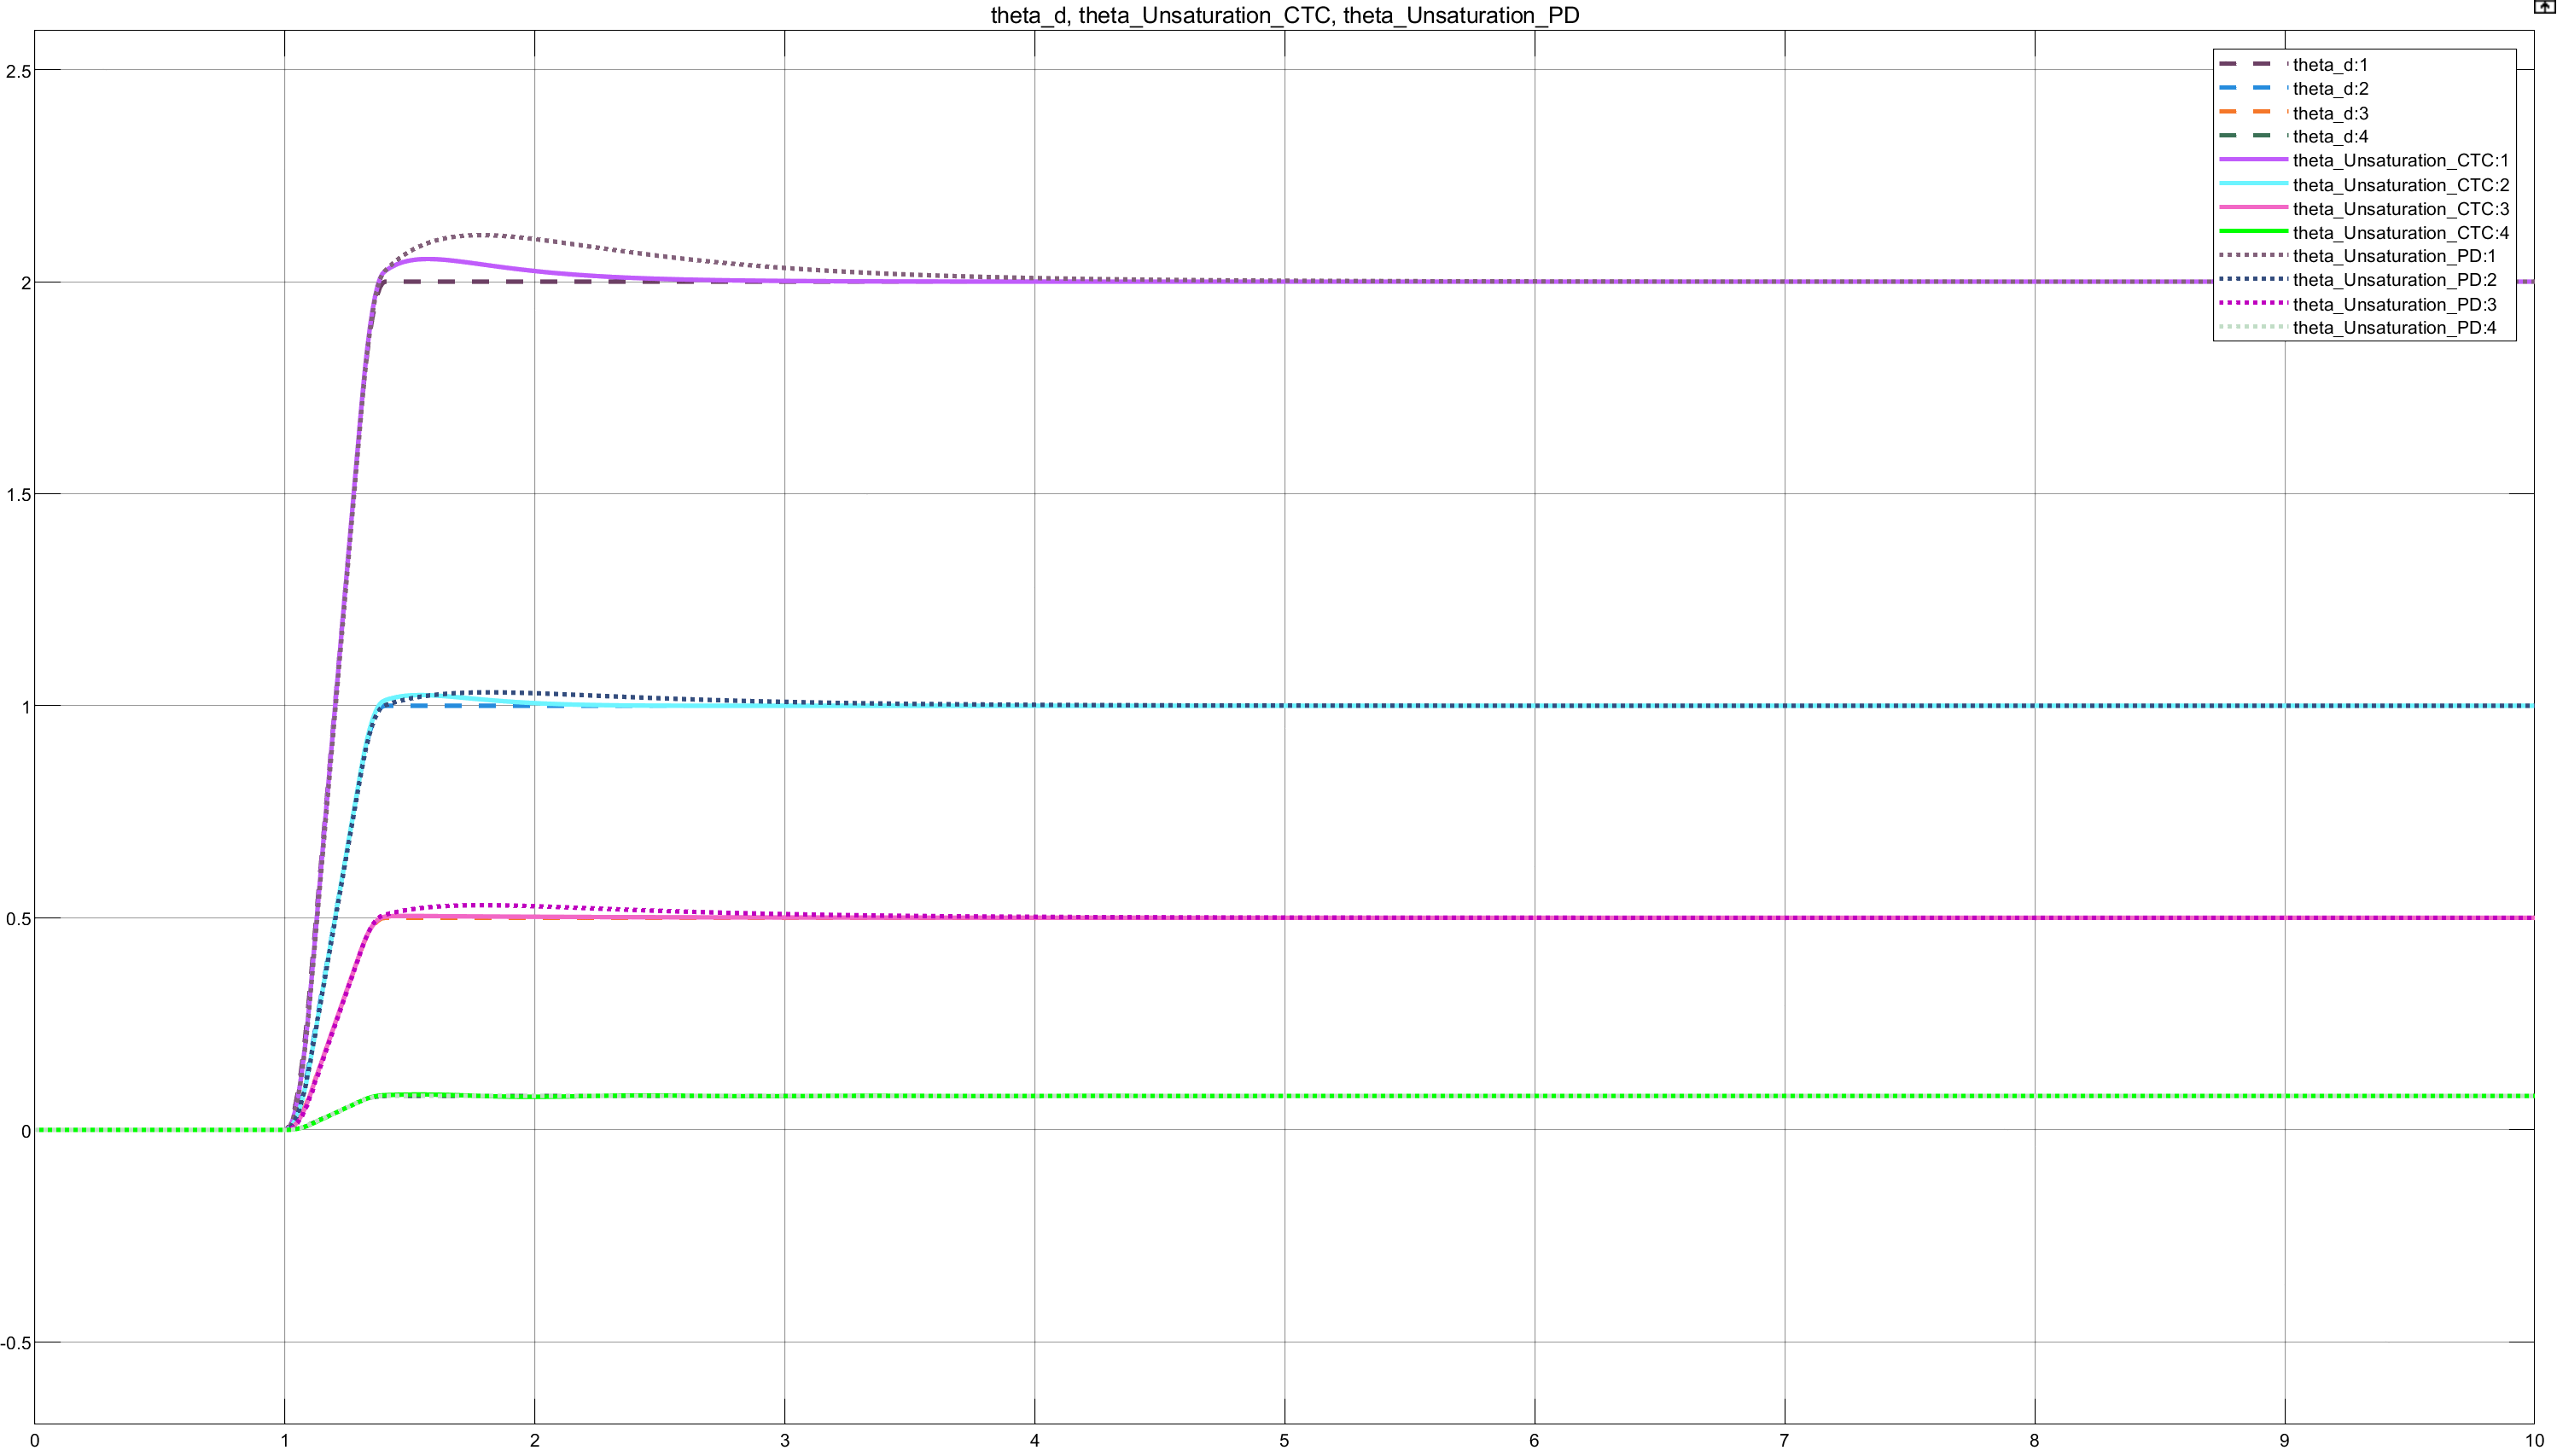
\includegraphics[width=0.92\textwidth]{c.png}
\caption{CTC vs.\ PD comparison (no saturation). \textbf{Dashed:} $\bm{\theta}_d$ (reference). \textbf{Solid:} CTC. \textbf{Dash-dot:} PD.}
\label{fig:c}
\end{figure}

\begin{resultbox}
\textbf{Observations:}
\begin{itemize}[nosep]
  \item \textbf{CTC}: tracks the reference almost perfectly --- smaller overshoot, faster response, and quicker convergence thanks to exact dynamic cancellation.
  \item \textbf{PD}: also converges to the reference, but with noticeably larger transient deviation and slower settling due to uncompensated Coriolis/centrifugal coupling.
  \item Both achieve zero steady-state error (PD benefits from gravity compensation).
  \item \textbf{Overall: CTC outperforms PD} in tracking accuracy, transient smoothness, and convergence speed, at the cost of higher computational complexity and model dependency.
\end{itemize}
\end{resultbox}

% ===================================================================
\section{Part (d): Torque Saturation}
\label{sec:d}
% ===================================================================

\textbf{Method.} Saturation blocks limit $|\bm{\tau}|\le[6000,2000,1000,100]^\top$ in all simulations. This is active throughout Parts (a)--(c).

\textbf{Results.} The effect of saturation is evident in the preceding sections:
\begin{itemize}[nosep]
  \item \textbf{Fig.~\ref{fig:a_theta}}: $\bm{\theta}$ (saturated) deviates from $\bm{\theta}_{\text{unsat}}$ (unsaturated) during the step transient --- most visible on joint~2, which exhibits a temporary dip when saturation clips the torque.
  \item \textbf{Fig.~\ref{fig:a_torque}}: the torque limits $[6000,2000,1000,100]^\top$ are reached during the transient, confirming that saturation is active.
  \item \textbf{Fig.~\ref{fig:b}}: under $\delta=+10\%$ plant perturbation with saturation active, tracking degrades from the combined effect of model mismatch and torque clipping.
\end{itemize}

\begin{resultbox}
\textbf{Finding:}
\begin{itemize}[nosep]
  \item Saturation is \textbf{not negligible} --- torque limits are hit during the step transient, causing visible tracking deviation, especially on joint~2.
  \item Joint~1 (base) has the highest torque demand; joint~2 is most visibly affected by clipping.
  \item Saturation slows the response and introduces transient tracking errors that would not exist under ideal unbounded actuation.
\end{itemize}
\end{resultbox}

% ===================================================================
\section{Conclusion}
% ===================================================================

Computed torque control achieves near-perfect tracking when the model is exact, with smaller overshoot, faster response, and quicker convergence than PD. Even with 10\% plant parameter mismatch (simulating aging), CTC continues to track effectively --- the PD feedback term provides sufficient correction. PD control trades peak accuracy for robustness and simplicity. Torque saturation is active during the step transient under the given limits $[6000,2000,1000,100]^\top$, causing visible tracking deviations (notably on joint~2); tighter limits would degrade performance further. Future work: adaptive/robust CT extensions and anti-windup schemes.

\end{document}
